\chapter{Capitolo 3: Albero Evolutivo}
Una delle sfide più importanti della bioinformatica, nonché l'obiettivo principale della filogenetica, è la costruzione degli alberi evolutivi.
\newline
Ricordando la definizione di albero, ovvero un grafo non orientato connesso e aciclico \cite{algoritmiEStruttureDati2}, \textit{L'albero evolutivo} o \textit{albero filogenetico} è un diagramma che rappresenta le relazioni evolutive tra i vari organismi \cite{buildingaphylogenictree}. La sua peculiarità consiste nel poterli costruire in base a dati genetici, genomici o morfologici, affinché si possano descrivere le relazioni che vi sono tra organismi viventi oppure tra specie estinte e specie viventi.
\newline
Gli alberi evolutivi possono essere suddivisi in due tipi, di seguito illustrati.
\newline
\begin{figure}[h!]
	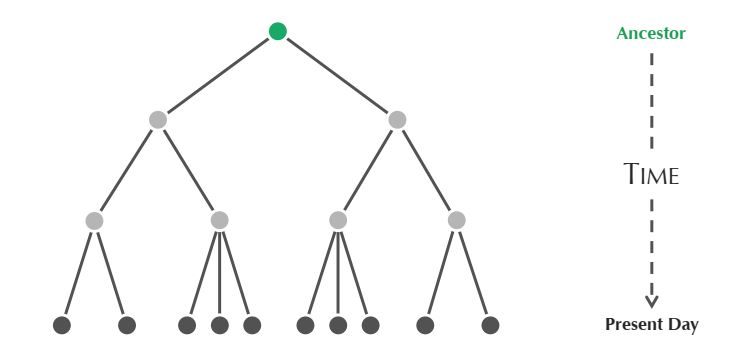
\includegraphics[width=\linewidth]{rooted_tree.jpg}
 	\caption{Albero radicato \cite{bioinfalganactivelearningapproachparttwo}.}
  	\label{fig:RootedTree}
\end{figure}
\newline
\textit{L'albero radicato} si sviluppa a partire da un nodo speciale, chiamato \textit{radice}

\newpage
Ordine dei capitoli:
\begin{itemize}
	\item Cap 3: alberi evolutivi;
	\item Cap 4: albero additivo;
	\item Cap 5: UPGMA (Unweighted Pair Group Method with Arithmetic Mean)
	\item cap 6: NEIGHBORJOINING
\end{itemize}

\begin{center}
\begin{forest}
for tree={circle,draw, l sep=32pt, s sep=33pt}
[k,red 
    [z,edge label={node[midway,left] {5}}
      [y,edge label={node[midway,left] {10}} ] 
      [l,edge label={node[midway,left] {12}}] 
      [m,edge label={node[midway,right] {7}}]
    ]
    [u,edge label={node[midway,right] {2}}
      [f,edge label={node[midway,left] {1}}] 
      [h,edge label={node[midway,left] {18}}] 
      [p,edge label={node[midway,right] {20}}]
  ] 
]
\end{forest}
%\label{fig:phyltree}
\end{center}